\section{Construct results by reusing pre-computed views}\label{sec: view_reuse}
In the previous section, we reviewed related works on how to maintain views in the context of data analysis tasks, where the views can be the model parameters, classification results and the results of linear algebra programs. However, given those predefined {\em views}, how to make those views usable for further data analysis tasks becomes another challenge, which is similar to traditional query rewriting using views problem \cite{halevy2001answering} in spirit.

In this section, \cite{hasani2018efficient} and part of \cite{gupta2015processing} are summarized, which aims at constructing approximate machine learning models by {\em reusing} the {\em pre-materialized} model parameters. The high-level idea is that the user issues a ``query'' on some subset of a dataset for building a machine learning model, which is then approximately (but efficiently) constructed by reusing and combining a set of ``relevant'' pre-materialized models. When building the model to answer users' requests, \cite{hasani2018efficient} proposes two different approaches to combining relevant pre-materialized models, i.e., {\em merging} the pre-materialized model parameters or combining their {\em coresets}, which incur different overhead and theoretical guarantee in terms of approximation. \eat{ but can deal with very general types of machine learning models, such as generalized linear models (GLMs), K-means and Guassian Mixture Models (GMMs).} However, only the first approach is employed in \cite{gupta2015processing}. Similar to query optimization problem, there might be multiple ways to derive the model for user's request, among which the one with minimal cost is expected in practice.

Considering the similarity between \cite{hasani2018efficient} and \cite{gupta2015processing}, in what follows, some basic concepts from \cite{hasani2018efficient} are introduced, which follow by the two different approaches to combining the pre-materialized models (as mentioned before) along with an algorithm on how to find the minimal-cost strategy for some limited type of queries and then follow by the sketched solutions to general queries. In the end, the differences between \cite{hasani2018efficient} and \cite{gupta2015processing} are highlighted.


\subsection{Basic concepts}
The dataset that \cite{hasani2018efficient} is dealing with is a relation $\textbf{D}$ with $n$ tuples (samples), $d$ attributes (features) $\bar{\textbf{a}} = \{\textbf{a}_1, \dots, \textbf{a}_d\}$, which may have hierarchical structures (e.g. attribute $city$ with hierarchical structure $City \rightarrow State \rightarrow Country$) and can be divided into feature attributes $\bar{\textbf{x}}$ and label attributes $\bar{\textbf{y}}$.

We can issue some queries to extract some tuples from $\textbf{D}$ via some predicates, such as {\em range based predicates} (e.g. $\textbf{a}_1 \in [lb, ub]$) and {\em dimension based predicates} (e.g. $\textbf{a}_2 = `c$') over some attributes, which are then used for training a machine learning model. In the following discussions, only range based predicates are considered. How to extend to general predicates is discussed later. 

The entire approach has two phases, i.e. ``pre-computing phase'' and ``running time phase''. During ``pre-computing phase'', a set of pre-materialized machine learning models $\mathcal{M} = \{M_1, M_2, \dots, M_n\}$ are prepared for answering user queries and each $M_i$ corresponds to a range based predicate over $\textbf{D}$ which is used to extract tuples from $D$ to construct $M_i$. In the following ``running time phase'', given a user query with a predicate, a set of candidate pre-materialized models are selected for approximately building the requested model.

\begin{example}\label{eg: two_phase_eg}
For example, given a relation $\textbf{D}=\{1,2,\dots, 1000\}$, in the pre-computing phase, the pre-materialized models $\{M_0, M_1, M_2, M_3, M_4\}$ can be built over the tuples from $\textbf{D}$ specified by the range predicate $P_0 = [100, 300], P_1 = [250, 500], P_2 = [500, 1000], P_3 = [300, 900], P_4 = [900, 1000]$. 

In the running time phase, a user query with predicate $q=[250, 1000]$ is submitted, for which we can combine $M_1$ and $M_2$ to compute the model for $q$.
\end{example}

\eat{As mentioned before, \cite{hasani2018efficient} targets at very general machine learning algorithms, such as K-means, GMMs and GLMs, the notations of which are briefly presented below:

\paragraph{K-means} K-means is an unsupervised clustering algorithm, which aims at computing a set of centroids $C$ from a set of data points $X$ and assigning each data point from $X$ to one of centroid in $C$ by minimizing the sum of square errors (SSE) with a similarity measure $d(*)$ in it:

\begin{equation}\label{eq: sse_k_means}
    SSE(X, C) = \sum_{\bar{x} \in X}d(\bar{x}, C)
\end{equation}

\paragraph{GMM} GMM is the probabilistic version of K-means, which is parameterized by a set of model parameters $\bar{\theta} = \{(w_1, \bar{\mu_1}, \Sigma_1), (w_2, \bar{\mu_2}, \Sigma_2), \dots, (w_k, \bar{\mu_k}, \Sigma_k)\}$ such that the probability of a data point $\bar{x}$ belonging to a cluster $i$ is computed by the probability density function of normal distribution and weighted by $w_i$, i.e.  $w_i\frac{exp(-\frac{1}{2}(\bar{x}-\bar{\mu}_i)^T\Sigma^{-1}(\bar{x}-\bar{\mu}_i))}{\sqrt{(2\pi)^k|\Sigma|}}$. The model parameters are derived during the training process with EM algorithm.

\paragraph{GLM} GLM includes a large class of typical linear classifiers such as logistic regression and support vector machine (SVM) and also typical regression methods, such as linear regression.}

\subsection{Constructing models for user query}
In this subsection, assuming that given a user query $q$ over a subset of $D$, i.e. $D_q$, the goal is to combine a set of candidate pre-materialized models $\mathcal{M}_q = \{M_1, M_2, \dots, M_r\}$ to construct the approximate model $\tilde{M}_q$ for answering $q$, which is achieved by two approaches i.e. {\em merging model} and {\em coreset construction}. 
% used to obtain an approximate model $\tilde{M}_q$ for $q$ are presented below. 

\subsubsection{Constructing by merging models}
% Suppose we can find a set of candidate pre-materialized machine learning models $\mathcal{M}_q (\subseteq \mathcal{M})$ usable for a user query $q$, 
{\em Merging model} approach simply merges the parameters from each model in $\mathcal{M}_q$ to compute the parameters of the approximate model $\tilde{M}_q$, which varies across different machine learning algorithms.

\paragraph{Merging model for K-means}
For K-means, each pre-materialized model stores a set of centroids as the parameters. Suppose the union of the centroids from $\mathcal{M}_q$ is $C_w$ and the cluster represented by a centroid $c_j$ in $C_w$ includes $w_j$ data points from $\textbf{D}$. Then K-means++ \cite{arthur2007k} runs over $C_w$ with weight $w_j$ for each centroid $c_j \in C_w$ to produce $k$ centroids as output, which will be a $O(log k)$-approximate model compared to the one constructed on $D_q$ directly and a $O(log^2k)$-approximate model compared to the theoretically optimal model on $D_q$.

\paragraph{Merging model for GMM}
The main takeaway of the solutions to K-means above is to cluster centroids from the candidate models with further invocations of the clustering algorithm, which, does not work for GMM, although GMM is a generalized model for K-means. This is because 1) the model parameters of GMM include mean vector, covariance matrix and a prior probability, which are far more complicated than K-means and far more expensive to estimate; 2) the merged model may be far away from the one built from the scratch. 

To overcome the issues above, the authors proposed an iterative approach to merge the GMM clusters from the candidate models $\mathcal{M}_q$, which starts by unioning all the cluster parameters from $\mathcal{M}_q$ (denoted by $\theta_q$) with the cluster parameters in the form of $(w_i, \bar{\mu}_i, \Sigma_i)$.
Then the most similar model pairs with parameters $(w_1, \bar{\mu}_1, \Sigma_1)$ and $(w_2, \bar{\mu}_2, \Sigma_2)$ are determined by Bhattacharyya distance \cite{bhattacharyya1943measure} (denoted by $D_B(*)$, see Equation \ref{eq: db_distance}), which are merged into a single cluster by following Equation \ref{eq: GMM_merging}.

\begin{equation}\label{eq: db_distance}
\begin{split}
    D_B(\bar{\mu}_1, \bar{\mu}_2, \Sigma_1, \Sigma_2) &=
    \frac{1}{8}(\bar{\mu}_1-\bar{\mu}_2)^T\Sigma^{-1}(\bar{\mu}_1 -\bar{\mu}_2) \\&+ \frac{1}{2}ln(\frac{|\Sigma|}{\sqrt{|\Sigma_1||\Sigma_2|}})\\
    \Sigma &= \frac{\Sigma_1 + \Sigma_2}{2}
\end{split}
\end{equation}

\begin{equation}\label{eq: GMM_merging}
    \begin{split}
        w &= w_1 + w_2\\
        \bar{\mu} &= \frac{1}{w}(w_1\bar{\mu}_1 + w_2\bar{\mu}_2)\\
        \Sigma &= \frac{w_1}{w}[\Sigma_1 + (\bar{\mu}_1 - \bar{\mu})^T(\bar{\mu}_1 -\bar{\mu})]\\
        &+\frac{w_2}{w}[\Sigma_2 + (\bar{\mu}_2 - \bar{\mu})^T(\bar{\mu}_2 -\bar{\mu})]
    \end{split}
\end{equation}

The merging process continues until there are exact $k$ clusters in the end.


\paragraph{Merging model for classifiers}
Suppose for each model $M_i \in \mathcal{M}_q$, the model parameter is $\theta(M_i)$, in order to derive the approximate model $\tilde{M}_q$ for $q$, the model parameters from $\mathcal{M}_q$ are simply averaged, i.e. $\theta(\tilda{M}_q) = \frac{1}{|\mathcal{M}_q|}\Sigma_{M \in \mathcal{M}_q}\theta(M)$, which, however, has been proven by \cite{zhang2012communication} to match the error rate of the model built from the scratch on $D_q$.

\paragraph{Merging model in \cite{gupta2015processing}} Recall that \cite{gupta2015processing} deals with different machine learning model from \cite{hasani2018efficient}, i.e. linear regression, Naive Bayes and logistic regression. Logistic regression belongs to GLM and thus the solution mentioned before for classifiers fit very well for it, which is thus not discussed here. But the authors of \cite{gupta2015processing} show that merging linear models or Naive Bayes models can end up with ``exact'' updated model parameters, which is presented below.

Recall that in Section \ref{sec: view_maintenance_model}, given a set of labeled training data points $D = \{\bar{x}_i, y_i\}_{i=1}^n$, the model parameters to be maintained for linear regression model are $X^TX$ and $X^T\bar{y}$, where $X$ and $\bar{y}$ are:

\begin{equation}
    X=\begin{bmatrix}
x_{11} & x_{12} &\dots &x_{1k}\\
x_{21} & x_{22} &\dots &x_{2k}\\
\dots\\
x_{n1} & x_{n2} &\dots &x_{nk}\\
\end{bmatrix}
=\begin{bmatrix}
\bar{x}_1^T\\
\bar{x}_2^T\\
\dots\\
\bar{x}_n^T\\
\end{bmatrix}
\end{equation}


\begin{equation}
    \bar{y} = \{y_1, y_2,\dots, y_n\}^T
\end{equation}

So $X^TX$ and $X^T\bar{y}$ have the following form:
\begin{equation}
    X^TX=\begin{bmatrix}
XX_{1,1} & XX_{1,2} &\dots XX_{1,k}\\
XX_{2,1} & XX_{2,2} &\dots XX_{2,k}\\
\dots\\
XX_{n,1} & XX_{n,2} &\dots XX_{n,k}\\
\end{bmatrix}=\begin{bmatrix}
\Sigma_{j=1}^nx_{j1}x_{j1} & \Sigma_{j=1}^nx_{j1}x_{j2} &\dots \Sigma_{j=1}^nx_{j1}x_{jk}\\
\Sigma_{j=1}^nx_{j2}x_{j1} & \Sigma_{j=1}^nx_{j2}x_{j2} &\dots \Sigma_{j=1}^nx_{j2}x_{jk}\\
\dots\\
\Sigma_{j=1}^nx_{jk}x_{j1} & \Sigma_{j=1}^nx_{jk}x_{j2} &\dots \Sigma_{j=1}^nx_{jk}x_{jk}\\
\end{bmatrix}
\end{equation}

\begin{equation}
    X^T\bar{y}=\begin{bmatrix}
Xy_{1}\\
Xy_{2}\\
\dots\\
Xy_{n}\\
\end{bmatrix}=\begin{bmatrix}
\Sigma_{j=1}^nx_{j1}y_{j}\\
\Sigma_{j=1}^nx_{j2}y_{j}\\
\dots\\
\Sigma_{j=1}^nx_{jk}y_{j}\\
\end{bmatrix}
\end{equation}

Given two models with materialized parameters $X_1^TX_1$, $X_1^T\bar{y}_1$ and $X_2^TX_2$, $X_2^T\bar{y}_2$ respectively which are constructed over two sets of data points $D_1$ and $D_2$, if $D_1 \bigcap D_2 = \Phi$, then they are merged as follows (suppose the materialized parameters for the merging model are $X^TX$, $X^T\bar{y}$ respectively):

\begin{equation}
\begin{split}
{XX}_{i,j} &= {X_1X_1}_{i,j} + {X_2X_2}_{i,j}\\
{Xy}_{i} &= {X_1y_1}_{i} + {X_2y_2}_{i}
\end{split}
\end{equation}

Otherwise,

\begin{equation}
\begin{split}
{XX}_{i,j} &= {X_1X_1}_{i,j} + {X_2X_2}_{i,j} - \Sigma_{\bar{x}_k \in D_1 \bigcap D_2}x_{ki}x_{kj} \\
{Xy}_{i} &= {X_1y_1}_{i} + {X_2y_2}_{i} - \Sigma_{\bar{x}_k \in D_1 \bigcap D_2}x_{ki}y_{k} 
\end{split}
\end{equation}


Similarly, for Naive Bayes model, since the values of $N_c$, $S_{jc}$ and $SS_{jc}$ are materialized for maintenance by referencing Section \ref{sec: view_maintenance_model}, given two models with materialized values $N1_c$, $S1_{jc}$, $SS1_{jc}$ and $N2_c$, $S2_{jc}$, $SS2_{jc}$ which are constructed over two sets of data points, $D_1$ and $D_2$, the materialized parameters (denoted by $N_c$, $S_{jc}$ and $SS_{jc}$) for the merging model are:

\begin{equation}
\begin{split}
N_c &= N1_c + N2_c-N_c'\\
S_{jc} &= S1_{jc} + S2_{jc}-S_{jc}'\\
SS_{jc} &= SS1_{jc} + SS2_{jc}-SS_{jc}'\\
\end{split}
\end{equation}

where $N_c'$, $S_{jc}'$ and $SS_{jc}'$ are materialized parameters for the model built on the data points in $D_1 \bigcap D_2$.

\subsection{Answering query by coreset}
Merging model approach is very efficient since it constructs the approximate model for the user query without having to access the data points but it lacks theoretical guarantee compared to the model built from the scratch for some machine learning algorithms, which can be alleviated by coreset approach.

Specifically, a weighted set of data points $C \subseteq \textbf{D}$ is a $\epsilon-$coreset for $D \subseteq \textbf{D}$ if $C \subseteq D$ and $(1-\epsilon)\phi(D) \leq \phi(C) \leq (1+\epsilon)\phi(D)$ where $\phi$ is the loss function (e.g. Equation \ref{eq: sse_k_means}) and $\phi(D)$ and $\phi(C)$ are the evaluation of $\phi$ over $D$ and $C$. Intuitively, the coreset is a subset of $D$, $C$ such that the machine learning model built on (weighted) $C$ and $D$ are close enough.

Recall that there are two computation phases for constructing approximate model for user query, i.e. {\em pre-computing phase} and {\em running time phase}. In {\em pre-computing phase}, the coreset is constructed for every pre-materialized model while in {\em running time phase}, the coresets derived from {\em pre-computing phase} are used to construct approximate model for user query, which are illustrated below.

\paragraph{Coreset in pre-computing phase} The coreset is constructed during {\em pre-computing phase} by one common strategy, i.e. sampling the data points proportional to their ``importance'' to the loss function $\phi$. The ``importance'' is quantified by a surrogate function which should be selected to 1) have good approximation ratio compared to the loss function $\phi$; 2) guarantee efficient computation; 3) be  agnostic about the optimal solution computed by $\phi$. So the surrogate function should be varied across different machine learning algorithms. For example, for K-means with loss function shown in Equation \ref{eq: sse_k_means}, given a set of data points $D_i$, the surrogate function is defined as follow:

\begin{equation}\label{eq: surrogate_function}
    p(x) = \frac{1}{2}\frac{1}{|D_i|} + \frac{1}{2}\frac{d(x, \mu(D_i))^2}{\Sigma_{x'\in D_i}d(x', \mu(D_i))^2}
\end{equation}

where $\mu(*)$ is used to compute the mean of all $D_i$. This equation is efficient since it only requires two passes over the entire $D_i$ to compute the importance for every $x \in D_i$. After computing the probability for every data point in $D_i$, we can do the probability sampling over the data points from $D_i$ to select $m$ data points where $m$ is the input sampling size, which guarantees that the result is $\epsilon-$coreset according to the proof in \cite{bachem2017scalable}.

\paragraph{Coreset in running time phase} There are two intriguing properties for coreset, which is beneficial to model construction in the running time phase. The first property is the {\em compositional} property, i.e. given the $\epsilon-$coresets $C_1$ and $C_2$ for two datasets $D_1$ and $D_2$, $C_1 \bigcup C_2$ should be also an $\epsilon-$coreset for $D_1 \bigcup D_2$, which can produce a coreset of large size for $D_q$ (the data points that the user query touches) if we union the coresets from all the candidate models from $\mathcal{M}_q$. 

To address this issue, we employ the second property of coreset, i.e. the size of an $\epsilon-$coreset simply depends on $\epsilon$ and a probability value $\delta$ but independent from the dataset size. For example, with the probability at least $1-\delta$, to generate a $\epsilon-$coreset for a K-means model, which should have the size at least $\Omega(\frac{dk+log\frac{1}{\delta}}{\epsilon^2})$ where $k$ is the cluster number and $d$ is the dimension number. Suppose each model in $\mathcal{M}_q$ has a coreset of size $m$, by following this property, the coreset construction algorithm is applied over the union of all the coresets from models in $\mathcal{M}_q$ (a set of size $m|\mathcal{M}_q|$) to generate a coreset of size $m$ for $D_q$.


\subsection{Optimizing the execution strategy}\label{sec: opt}
In the previous subsection, we assume that the candidate model set $\mathcal{M}_q$ is given for a user query $q$ and analyze how to construct approximate models with $\mathcal{M}_q$ with {\em merging model} approach or {\em coreset} approach. However, in practice, there can be multiple possible options for $\mathcal{M}_q$. For example, let us revisit Example \ref{eg: two_phase_eg}, to construct model for query $q$, there are two candidate model sets. The first one is $\{M_1, M_2\}$, which exactly covers the range predicate of $q$ and thus can be combined directly to build the model for $q$. The other option is to train an auxiliary model $M'$ for the range $[250, 300]$ and combine $M'$, $M_3$ (with predicate $[300, 900]$) and $M_4$ (with predicate $[900, 1000]$) for the same purpose. 

\paragraph{Cost measure} To compare those different options and thus find the best ones, the authors introduce cost measures for the cost of building model from the scratch $C_{build}$, combining models with {\em merging model} approach (denoted by $C_{merge}$) or {\em coreset} approach (denoted by $C_{coreset}$) to evaluate the total overhead for each option. For Example \ref{eg: two_phase_eg}, suppose {\em merging model} approach is used, then the cost of the first option and second option above will be $C_{merge}(M_1) + C_{merge}(M_2)$ and $C_{build}(M') + C_{merge}(M_3) + C_{merge}(M_4)$ respectively. 

\paragraph{Building execution strategy graph} Based on the cost measure, the problem of determining the min-cost strategy is formulated as the shortest path problem in the {\em execution strategy graph}, where the node set is composed of the distinct lower bound and upper bound values of all the range based predicates from the pre-materialized models as well as the query (with range based predicate $[lb, ub]$) while weighted edge is built from node $a$ to node $b$ such that $a < b$. The weight on every edge from node $a$ to $b$ represents the cost to ``cover'' the interval $[a,b]$, which depends on whether there exists a pre-materialized model built over this interval. If not, then the weight is $C_{build}([a,b])$. Otherwise, the weight will be $C_{merge}([a,b])$ for merging model approach or $C_{merge}([a,b]) + C_{coreset}([a,b])$ for coreset approach. Then we run Dijkstra's algorithm over the graph to determine the shortest path from the node $lb$ to the node $ub$. Note that before the graph constructing process, only the ``relevant'' pre-materialized models are considered, which have predicates fully covered by the query predicate. Let us revisit Example \ref{eg: two_phase_eg} to see how the graph is constructed.

\begin{example}
In Example \ref{eg: two_phase_eg}, $M_0$ is not relevant model for $q$ since the corresponding range based predicate $[100, 300]$ is not a subset of the predicate $[250, 1000]$ in the query, which is thrown away while other models are all relevant. For the predicates of the relevant models and the query predicates, their lower bound and upper bound values compose the following set: $\{250, 300, 500, 900, 1000\}$, each of which becomes a node in the graph. Assuming the the merging model approach is used, the edges and corresponding weights are then constructed by following the rules mentioned above, which ends up with a graph in Figure \ref{fig:min_cost_graph}. Finally, Dijkstra's algorithm is applied over this graph to derive the shortest path from the node 250 to the node 1000 and thus determine the option with minimal cost.


% \begin{figure}[t]
% \begin{center}
% \begin{tikzpicture}[grow'=up,scale=0.75]
% % \tikzset{vertex/.style = {shape=circle,draw,minimum size=1.5em}}
% % \tikzset{edge/.style = {->,> = latex'}}
% % vertices
% \node (1) at (-2,0) {$250$};
% \node (2) at (6,0) {$300$};
% \node (3) at (-4,4) {$500$};
% \node (4) at (2,8) {$900$};
% \node (5) at (8,4) {$1000$};
% %edges
% % \draw[edge] (1) to (3);
% % \path[->]
% % (1) edge[bend left] node[swap] {$\neg$} (2)
% % (2) edge[bend left] node {$\neg$} (1);
% \scriptsize{
% \draw[->] (1) --(3) node[pos=0.5,left]{$C_{combine}([250, 500])$}; 
% \draw[->] (1) --(2) node[pos=0.5,below]{$C_{build}([250, 300])$}; 
% \draw[->] (2) --(3) node[pos=0.6,right]{$C_{build}([300, 500])$}; 
% \draw[->] (3) --(5) node[pos=0.5,above]{$C_{combine}([500, 1000])$};
% \draw[->] (2) --(4) node[pos=0.15,above]{$C_{combine}([300, 900])$};
% \draw[->] (4) --(5) node[pos=0.7,right]{$C_{combine}([900, 1000])$};
% \draw[->] (3) --(4) node[pos=0.5,left]{$C_{build}([500, 900])$};
% \draw[->] (1) --(5) node[pos=0.2,above]{$C_{build}([250, 1000])$};
% \draw[->] (2) --(5) node[pos=0.5,right]{$C_{build}([300, 1000])$};
% \draw[->] (1) --(4) node[pos=0.7,above]{$C_{build}([250, 900])$};}
% % \draw[edge] (2) to (3); 
% % \draw [->] (-0.4,0.3) arc (10:330:20pt);
% \end{tikzpicture}
% \end{center}
% \caption{Graph to determining the option with minimal cost}
% \label{fig:min_cost_graph}
% \end{figure}


\begin{figure}[t]
\begin{center}
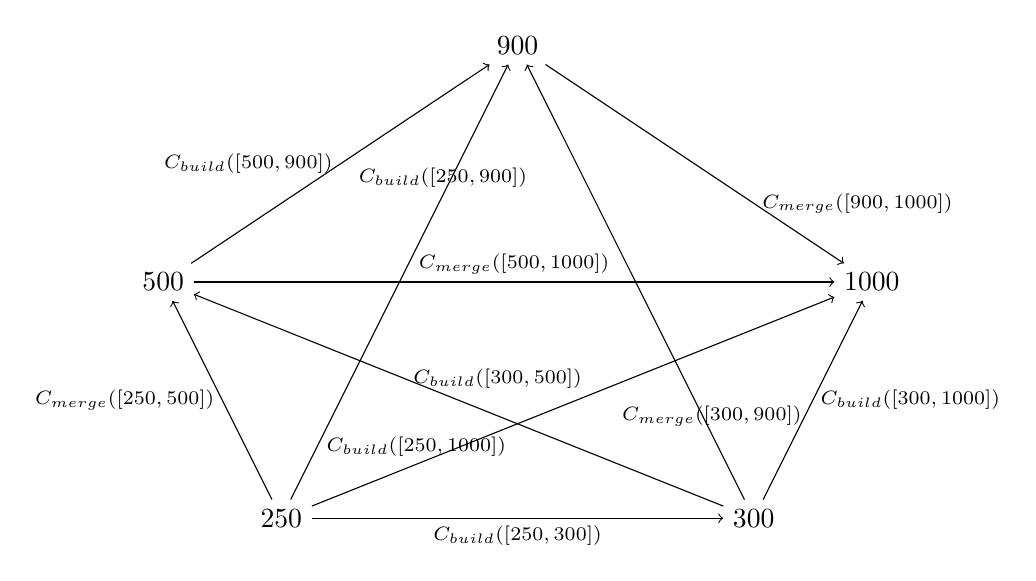
\begin{tikzpicture}[grow'=up,scale=0.75]
% \tikzset{vertex/.style = {shape=circle,draw,minimum size=1.5em}}
% \tikzset{edge/.style = {->,> = latex'}}
% vertices
\node (1) at (-2,0) {$250$};
\node (2) at (6,0) {$300$};
\node (3) at (-4,4) {$500$};
\node (4) at (2,8) {$900$};
\node (5) at (8,4) {$1000$};
%edges
% \draw[edge] (1) to (3);
% \path[->]
% (1) edge[bend left] node[swap] {$\neg$} (2)
% (2) edge[bend left] node {$\neg$} (1);
\scriptsize{
\draw[->] (1) --(3) node[pos=0.5,left]{$C_{merge}([250, 500])$}; 
\draw[->] (1) --(2) node[pos=0.5,below]{$C_{build}([250, 300])$}; 
\draw[->] (2) --(3) node[pos=0.6,right]{$C_{build}([300, 500])$}; 
\draw[->] (3) --(5) node[pos=0.5,above]{$C_{merge}([500, 1000])$};
\draw[->] (2) --(4) node[pos=0.15,above]{$C_{merge}([300, 900])$};
\draw[->] (4) --(5) node[pos=0.7,right]{$C_{merge}([900, 1000])$};
\draw[->] (3) --(4) node[pos=0.5,left]{$C_{build}([500, 900])$};
\draw[->] (1) --(5) node[pos=0.2,above]{$C_{build}([250, 1000])$};
\draw[->] (2) --(5) node[pos=0.5,right]{$C_{build}([300, 1000])$};
\draw[->] (1) --(4) node[pos=0.7,above]{$C_{build}([250, 900])$};}
% \draw[edge] (2) to (3); 
% \draw [->] (-0.4,0.3) arc (10:330:20pt);
\end{tikzpicture}
\end{center}
\caption{Graph to determining the option with minimal cost}
\label{fig:min_cost_graph}
\end{figure}

\end{example}

\paragraph{Building execution strategy graph in \cite{gupta2015processing}} Observe that when combining two or models to construct new model for the user query in \cite{hasani2018efficient}, more and more data points from $\textbf{D}$ are included rather than removed. For example, in Example \ref{eg: two_phase_eg}, we need to combine the model $M_3$ and $M_4$ toward the construction of the model for query $q$, $M_q$ and the data points that $M_3$ and $M_4$ are built on, i.e. the data points in $[300, 900]$ and $[900, 1000]$, are unioned, indicating that those data points are necessary to build $M_q$.  In contrast, during the combinations of pre-materialized models for linear regression and Naive Bayes, \cite{gupta2015processing} can also handle the case where the unnecessary data points are removed from those models, which thus result in different concepts of {\em relevant} pre-materialized models and thus different ways to construct the execution strategy graphs.

Given a query $q$ with a range based predicate $P_q = [lb,ub]$, a pre-materialized model $M_i$ with a range based predicate $P_i$ is relevant to $q$ if the intersection of $P_i$ and $P_q$ is not empty or the intersection of $P_i$ and the range based predicate of some relevant pre-materialized models is not empty. 

\begin{example}\label{eg: relevant_models}
For example, if a query $q'$ has range predicate $[100, 500]$, for the pre-materialized models provided in Example \ref{eg: two_phase_eg}, the relevant models should include all of them. Note that although the range predicate of $M_4$ ($[900, 1000]$) does not share the same data point as the range predicate of $q'$ ($[100, 500]$), it has common data with the range predicate of $M_3$, which is a relevant model.
\end{example}

After the relevant pre-materialized models are determined, the execution strategy graph is constructed in the same way as \cite{hasani2018efficient} does. For example, in Example \ref{eg: relevant_models}, the graph is shown in Figure \ref{fig:min_cost_graph2}.

\begin{figure}[t]
\begin{center}
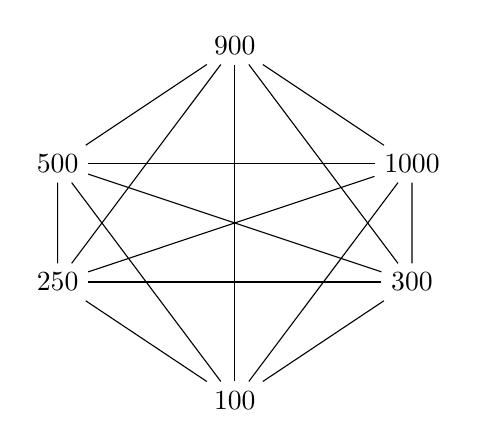
\begin{tikzpicture}[grow'=up,scale=0.75]
% \tikzset{vertex/.style = {shape=circle,draw,minimum size=1.5em}}
% \tikzset{edge/.style = {->,> = latex'}}
% vertices
\node (0) at (1,-2) {$100$};
\node (1) at (-2,0) {$250$};
\node (2) at (4,0) {$300$};
\node (3) at (-2,2) {$500$};
\node (4) at (1,4) {$900$};
\node (5) at (4,2) {$1000$};
%edges
% \draw[edge] (1) to (3);
% \path[->]
% (1) edge[bend left] node[swap] {$\neg$} (2)
% (2) edge[bend left] node {$\neg$} (1);
\scriptsize{
\draw[-] (1) --(3) ;%node[pos=0.5,left]{$C_{merge}([250, 500])$}; 
\draw[-] (1) --(2) ; 
\draw[-] (2) --(3) ; 
\draw[-] (3) --(5) ;
\draw[-] (2) --(4) ;
\draw[-] (4) --(5) ;
\draw[-] (3) --(4) ;
\draw[-] (1) --(5) ;
\draw[-] (2) --(5) ;
\draw[-] (1) --(4) ;
\draw[-] (0) --(1) ;
\draw[-] (0) --(2) ;
\draw[-] (0) --(3) ;
\draw[-] (0) --(4) ;
\draw[-] (0) --(5) ;
}
% \draw[edge] (2) to (3); 
% \draw [->] (-0.4,0.3) arc (10:330:20pt);
\end{tikzpicture}
\end{center}
\caption{Execution strategy graph in \cite{gupta2015processing}}
\label{fig:min_cost_graph2}
\end{figure}

Due to the space limit, the edge weights are not shown in Figure \ref{fig:min_cost_graph2}, which is computed similarly compared to Figure \ref{fig:min_cost_graph}. Then Dijkstra's algorithm is applied to derive the shortest path from $100$ to $500$. Note that different from Figure \ref{fig:min_cost_graph}, the edges in Figure \ref{fig:min_cost_graph2} become undirected, which indicates that for an edge $i-j$ ($i < j$), the path can traverse it by either direction. The traversal direction over an edge represents addition or removal of the model over the corresponding data points. For example, one potential minimal path $\mathcal{P}$ in Figure \ref{fig:min_cost_graph2} from $100$ to $500$ would be $100\rightarrow 300 \rightarrow 250 \rightarrow 500$ since $M_0$ and $M_1$ are built on the range predicate $[100, 300]$ and $[250, 500]$ respectively, which can be reused to reduce the cost. The data points within $[100, 300]$ and $[250, 500]$ are included for model construction for $q'$, which is also reflected in the direction of the path $\mathcal{P}$, i.e. $100 \rightarrow 300$ and $250 \rightarrow 500$. However, since there is an overlap between the two range predicates, the data points within $[250, 300]$ should be removed (see the edge direction $300\rightarrow250$ in the path $\mathcal{P}$), which is achieved by constructing another model from the scratch over $[250, 300]$ and combining it with $M_0$ and $M_1$ to remove the effect of the duplicated data points in $[250, 300]$.

\subsection{selecting models for pre-materialization}\label{sec: select_models}
The authors of \cite{hasani2018efficient} also explored how to select models for pre-materialization given a set of queries from a workload, which is resolved with two stages, i.e. {\em candidate generation step} to generate a set of possible models and {\em candidate selection step} to retain the best models from the previous step according to a utility metric.

In the {\em candidate generation step}, given a set of queries $\{Q_1, Q_2, \dots, Q_m\}$ and the corresponding predicates $\{[lb_1, ub_1], [lb_2, ub_2], \dots, [lb_m, ub_m]\}$, the candidate predicate $[l, u]$ is considered such that 1) $l \leq u$; 2) $l, u \in \{lb_1, ub_1, lb_2, ub_2, \dots, lb_m, ub_m\}$; 3) $[l, u]$ is included by at least one $[lb_i, ub_i]$ ($i=1,2,\dots, m$).

In the {\em candidate selection step}, the utility evaluation of a set of candidate pre-materialized models $\mathcal{M} = \{M_1, M_2, \dots, M_k\}$ is determined by the difference between the sum of the cost of answering query $Q_i$ ($i=1,2,\dots, m$) using $\mathcal{M}$ and the sum of the cost to evaluate every $Q_i$ without pre-materializing any models, in which the cost is computed by the shortest path in the graph as constructed in Section \ref{sec: opt}. Then $L$ models with highest utility are selected.

\subsection{For arbitrary queries}
The previous subsections only consider a type of queries with predicates over one attribute, which cannot represent the general cases in practice since the predicates of the queries may touch multiple attributes or hierarchical attributes, the complexity of which can be NP-hard. Given the cost measure proposed in Section \ref{sec: opt}, how to adapt the search algorithm for optimal strategy and how to select the models for pre-materialization for arbitrary queries are introduced below.

In terms of optimally selecting the pre-materialized models under the existence of multiple attributes in the query predicates, the selected pre-materialized models should cover the data points from $\textbf{D}$ touched by the query and incur minimal cost, which is an instantiation of set cover problem. To derive a set of optimal or nearly optimal pre-materialized models efficiently, a greedy algorithm is proposed, which originates from the greedy algorithm for the set cover problem and sketched as follows: Given a user query $q$, which retrieves a set of data points from $\textbf{D}$, $D_q$, a set of candidate pre-materialized models $\mathcal{M}_q$ can be determined. Then under the cost model proposed in Section \ref{sec: opt}, the model $M \in \mathcal{M}_q$ covering the most data points from $D_q$ with least cost is chosen and the data points covered by $M$ is removed from $D_q$, which proceeds iteratively until $D_q$ becomes empty.

In order to select models for pre-materialization for arbitrary queries, the {\em candidate generation step} and the {\em candidate selection step} are still needed. In the {\em candidate generation step}, all the pairs of $(Q_i, Q_j)$ from the workload which cover $D_i$ and $D_j$ from $\textbf{D}$ respectively are used to compose four candidate models over four set of data points respectively, i.e. $D_i, D_j, D_i \bigcup D_j, D_i \bigcap D_j$. Then same as Section \ref{sec: select_models}, in the {\em candidate selection step}, the $L$ models with the highest utility are chosen for pre-materialization.

\subsection{Experimental results}

The authors in both \cite{gupta2015processing} and \cite{hasani2018efficient} conduct extensive experiments, which indicate the feasibility of model reuse in terms of speeding up computation as well as preserving the accuracy. In this subsection, only one set of experiments are presented due to the space limit, which show similar effect to other experiments. In the experiments, synthetic queries are used, which are generated by randomly picking up the query predicates while the entire datasets are partitioned multiple partitions randomly and one pre-materialized model is built over each of them. 

The experimental results are shown in Figure \ref{fig:model_reuse}, in which the x-axes of the four sub-figures represent the number of pre-materialized models and thus the number of partitions. The y-axes of Figure \ref{fig:model_reuse1} and Figure \ref{fig:model_reuse3} are the speed-ups compared to constructing models from the raw dataset while the ones of Figure \ref{fig:model_reuse2} and Figure \ref{fig:model_reuse4} represents accuracy approximation rate of the combined models relative to the models built from the scratch, which is termed as ``difference in accuracy'' and lies in the interval $[0,1]$. Smaller y value indicates better approximation. Note that both merging model approach and coreset approach outperform the the approach to building models from the scratch by orders of magnitude while the speed-ups have no impact over the model accuracy, which thus justifies the potential of the two approaches in practice.

\begin{figure}[h]
\captionsetup[subfigure]{width=1\textwidth}
     \centering
    \begin{subfigure}{0.2\textwidth}
        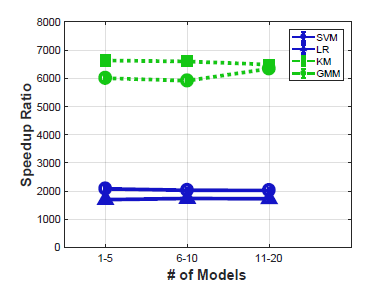
\includegraphics[height = 1.2\textwidth, width=1.2\textwidth]{Figures/model_reuse_merge_model_speed_up.png}
        \caption{Speed-ups for merging model approach}
        \label{fig:model_reuse1}
    \end{subfigure}
    \hfill
    % \hspace{1.5cm}
    \begin{subfigure}{0.2\textwidth}
        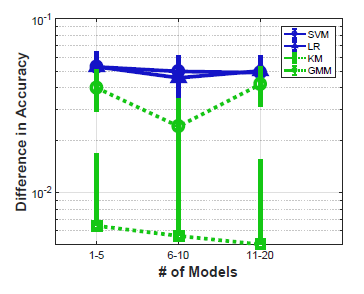
\includegraphics[height = 1.2\textwidth, width=1.2\textwidth]{Figures/model_reuse_merge_model_accuracy.png}
    \caption{Accuracy approximation for merging model approach}
    \label{fig:model_reuse2}
    \end{subfigure}
    \hfill
    \begin{subfigure}{0.2\textwidth}
        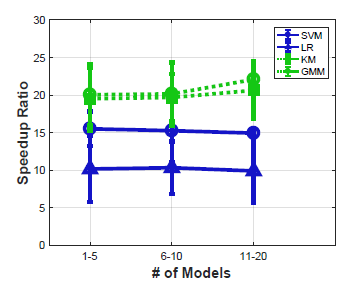
\includegraphics[height = 1.2\textwidth, width=1.2\textwidth]{Figures/model_reuse_coreset_speed_up.png}
    \caption{Speed-ups for coreset approach}
    \label{fig:model_reuse3}
    \end{subfigure}
    \hfill
    \begin{subfigure}{0.2\textwidth}
        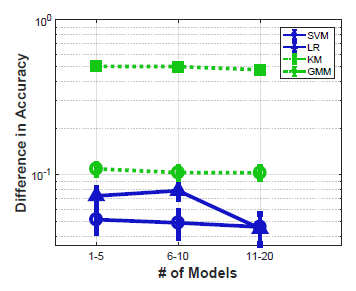
\includegraphics[height = 1.2\textwidth, width=1.2\textwidth]{Figures/model_reuse_coreset_accuracy.png}
    \caption{Accuracy approximation for coreset approach}
    \label{fig:model_reuse4}
    \end{subfigure}
    \caption{Experimental results of model reuse strategy}
    \label{fig:model_reuse}
\end{figure}


\subsection{Discussions}
In this section, we summarized the major contributions of \cite{gupta2015processing} and \cite{hasani2018efficient}, which borrows some ideas from query rewriting using views to exploit pre-materialized models to efficiently construct the machine learning model over the data points specified by user queries instead of training from the scratch. For a specific machine learning model $M$, the way to combine the pre-materialized instantiated $M$ over different training data points is closely related to the characteristics of incremental maintenance over $M$. As highlighted in the Section \ref{sec: maintain_views}, the incremental updates over linear regression and Naive Bayes can be either addition or removal of data points used for model construction, whose effect can thus be included or excluded when constructing the model for user queries by applying the solutions in \cite{gupta2015processing}. In contrast, other types of machine learning models lacking the power of incrementally removing the effect of some data points are thus suitable for the solutions of \cite{hasani2018efficient}.

\paragraph{Relationship to query rewriting using views} Query rewriting using views problem is a well-known research problem in database community \cite{halevy2001answering}. Some works have been focusing on optimizing the query response time with materialized views in the case of conjunctive queries \cite{chandra1977optimal, chaudhuri1995optimizing, pottinger2000scalable, afrati2007using}, aggregate queries \cite{cohen2007deciding, cohen1999rewriting, srivastava1996answering, galindo2001orthogonal}, nested queries \cite{zaharioudakis2000answering}, which play an important role in query optimization and data integration \cite{halevy2001answering}. However, those works only focus on propagating updates through the traditional database operations, i.e. the relation-algebra-based operations, which only covers a small portion of the operations used in current data analysis tasks. As mentioned before, in \cite{gupta2015processing} and \cite{hasani2018efficient}, the pre-materialized machine learning models and the user requests to train a new model are regarded as views and queries respectively such that the same ideas from traditional query rewriting using views problem are usable, i.e. {\em reuse} the pre-computation result for performance gains.

\paragraph{Relationship to transfer learning} In machine learning community, training a model with high accuracy requires a large volume of high-quality labeled data and advanced computation resources, which are usually not available for users.  So the idea of {\em transfer learning} emerges, which gives a chance to users to use some publicly available pre-trained machine learning models, such as caffe Model Zoo \cite{jia2015caffe}, TensorFlow models\footnote{https://github.com/tensorflow/models}, Mask R-CNN \cite{matterport_maskrcnn_2017}, etc., in their own applications. But considering the distribution deviation between the training data for pre-trained models and the training data in users' target applications, it is essential to select and combine those pre-trained models to fit users' requirement. Under the assumption that users usually have no access to the training data for pre-trained models due to privacy issues or storage capacity issue, this problem has been explored by researchers in transfer learning domain \cite{eaton2008modeling}, in which they also build a graph to measure the similarities between pre-trained models and model to be built based on the users' requests. To construct the model for the user query, the effect of those pre-trained models are combined according to the similarity measures  without caring about whether the pre-trained models are built on the relevant data for user query or not. It might be a good opportunity to complement \cite{eaton2008modeling} and other similar works on transfer learning by excluding the effect of irrelevant data to the user query when combining pre-materialized models just like \cite{gupta2015processing} did when the training data sets for those pre-trained models are accessible.
% So \cite{hasani2018efficient} and \cite{gupta2015processing} pave the way towards achieving this goal.

% \subsection{Differences between \cite{hasani2018efficient} and \cite{gupta2015processing}}
% Both \cite{hasani2018efficient} and \cite{gupta2015processing} mainly deal with queries with range predicates over one attribute, which both determine the minimal-cost execution strategy by building the execution strategy graph with relevant pre-materialized models and the user query (introduced in Section \ref{sec: opt}) and then applying Dijkstra's algorithm over that. The differences between \cite{hasani2018efficient} and \cite{gupta2015processing} lie in the concept of relevant pre-materialized models for a given query and thus the construction of the execution strategy graph.